\documentclass[10pt, conference]{IEEEtran}
\usepackage[pdftex]{graphicx}

\usepackage[ruled,lined]{algorithm2e}
\usepackage{amsfonts,amssymb,amsmath, tikz,kotex,mathtools}
\usepackage{microtype,xspace}
\usepackage{url,color,multirow}
\urldef{\mailsa}\path|{alfred.hofmann, ursula.barth, ingrid.haas, frank.holzwarth,|
\urldef{\mailsb}\path|anna.kramer, leonie.kunz, christine.reiss, nicole.sator,|
\urldef{\mailsc}\path|erika.siebert-cole, peter.strasser, lncs}@springer.com|    
\usepackage{stmaryrd}
\newcommand{\mtt}[1]{\texttt{\small #1}}
\newcommand{\msf}[1]{{\sf\small #1}}
\newcommand{\oldsafe}{{SAFE 1.0}\xspace}
\newcommand{\safe}{{SAFE~2.0}\xspace}
\newcommand{\htmldebug}{{\sf\small HTML Debugger}\xspace}

\hyphenation{op-tical net-works semi-conduc-tor}
\begin{document}
\title{\hspace*{-.7em}
Analysis of JavaScript Web Applications\\ Using \safe}

\author{\IEEEauthorblockN{Jihyeok Park}
\IEEEauthorblockA{KAIST\\
{ jhpark0223@kaist.ac.kr}}
\and
\IEEEauthorblockN{Yeonhee Ryou}
\IEEEauthorblockA{KAIST\\
{ ryou770@kaist.ac.kr}}
\and
\IEEEauthorblockN{Joonyoung Park}
\IEEEauthorblockA{KAIST\\
{ gmb55@kaist.ac.kr}}
\and
\IEEEauthorblockN{Sukyoung Ryu}
\IEEEauthorblockA{KAIST\\
{ sryu.cs@kaist.ac.kr}}}
\maketitle


\begin{abstract}
JavaScript has been the language for web applications, and
the growing prevalence of web environments in various devices
makes JavaScript web applications even more ubiquitous.
However, because JavaScript and web environments are
extremely dynamic, JavaScript web applications are often
vulnerable to type-related errors and security attacks.
To lessen the problem, researchers have developed various analysis
techniques in different analyzers, but such analyzers are not especially
aimed for ease of use by analysis developers.  In this paper, we present \safe, a scalable
analysis framework for ECMAScript especially designed as a playground
for advanced research in JavaScript web applications.  \safe is
light-weight, which supports configurability, extensibility, and
debuggability.
\end{abstract}


\section{Introduction}
JavaScript has become the language for web applications, but
JavaScript web applications are often vulnerable to programmer
errors and security attacks.  Because JavaScript provides
extremely functional and dynamic features and high portability
with web environments, web developers build web applications
mostly in JavaScript these days.  However, the characteristics
that brought the prevalent uses of JavaScript web applications
also introduce difficulties in building correct web applications.
The extremely functional and dynamic features make programs
hard to write correctly and hard to reason about.
Also, the dynamism and portability of web environments make
web applications vulnerable to security attacks.


To help JavaScript developers build correct programs, researchers
have developed analyzers that support various analysis techniques,
but they are not especially designed for usability.
SAFE\footnote{\url{http://plrg.kaist.ac.kr/redmine/projects/jsf/repository}}~\cite{Lee12}
is a scalable analysis framework for ECMAScript, and it has adopted recent research results incrementally.
While more analysis techniques make SAFE more featureful,
they make the code base of SAFE large and complex, which makes it
difficult for new users to understand the code base.
TAJS\footnote{\url{https://github.com/cs-au-dk/TAJS}}~\cite{TAJSDETER}
is a dataflow analysis for JavaScript that infers type information and call graphs.
It provides an analysis technique as a whole with an option instead of as
configurable components;
for example, the \mtt{-determinacy} option enables the techniques described in~\cite{TAJSDETER}.
WALA\footnote{\url{http://wala.sourceforge.net/wiki/index.php}}~\cite{Schafer13}
was originally developed for pointer analysis of Java programs, and it
also supports flow-insensitive pointer analysis of JavaScript programs.
Because WALA aims to support analysis of multiple programming languages,
the source code repository is huge with many packages.
While SAFE, TAJS, and WALA are mainly static analyzers possibly using dynamic information,
Jalangi\footnote{\url{https://github.com/SRA-SiliconValley/jalangi}}~\cite{Sen13}
is a dynamic analysis framework for JavaScript, which may miss many execution flows.
It provides simple dynamic analyzers like a taint analyzer as example uses of the framework.


Let us consider SAFE more closely\footnote{
Note that one of the authors is a main developer of SAFE.}.  It was first designed to analyze pure
JavaScript benchmarks~\cite{Lee12}.  It provides a default static analyzer
based on the abstract interpretation framework, and it supports
flow-sensitive and context-sensitive analyses of JavaScript
programs.  It performs several preprocessing steps on JavaScript code to
address quirky semantics of JavaScript such as the \mtt{with}
statement~\cite{dls13}.
%, and that part has been used by other researchers~\cite{jsai,kjs}.
It was then extended to model web application execution environments
of various browsers~\cite{safewapp} with HTML/DOM tree abstraction,
and it supports analysis of interactions between JavaScript code
and native functions in platform-specific libraries by using automatic
modeling of library functions from API specifications~\cite{SAFEWAPI}.
Recent extensions of SAFE include aggressive integration of
soundy~\cite{soundy} analysis.  Instead of analyzing the entire concrete
behaviors of programs, it supports an analysis of partial
programs by using approximate call graphs from WALA~\cite{asewala}.
It also utilizes dynamic information statically to focus on specific
environments like specific browser versions~\cite{safehybrid}.
The more advanced analysis techniques SAFE integrates,
the more difficult it is for SAFE users to understand the SAFE code base.

\setcounter{figure}{1}
\begin{figure*}[t]
\centering
\begin{tabular}{c}
\begin{minipage}{.95\textwidth}
\footnotesize
\begin{verbatim}
val commands: List[Command] = List(CmdParse, CmdASTRewrite, CmdCompile, CmdCFGBuild, CmdAnalyze,
                                   CmdBugDetect, CmdHelp)
var phases: List[Phase] = List(Parse, ASTRewrite, Compile, CFGBuild, Analyze, BugDetect, Help)
\end{verbatim}
\end{minipage}
\\[1.5em]
{\small (a) Add a new command and a new phase to the lists of available
commands and phases, respectively, in \mtt{Safe.scala}}
\\[1em]
\begin{minipage}{.95\textwidth}
\footnotesize
\begin{verbatim}
case object CmdBugDetect extends CommandObj("bugDetect", CmdAnalyze >> BugDetect) {
  override def display(cfg: CFG): Unit = println(cfg.toString(0))
}
\end{verbatim}
\end{minipage}
\\[1em]
{\small (b) Add the new command by specifying its name and phases in \mtt{Command.scala}}
\\[1em]
\begin{minipage}{.95\textwidth}
\footnotesize
\begin{verbatim}
case object BugDetect extends PhaseObj[(CFG, Int, CallContext), BugDetectConfig, CFG] {
  val name: String = "bugDetector"
  val help: String = "Detect possible bugs in JavaScript source files."
  def apply(in: (CFG, Int, CallContext), safeConfig: SafeConfig, config: BugDetectConfig): Try[CFG] = {
    val (cfg, _, _) = in
    // Bug detector implementation here.
    Success(cfg)
  }
  def defaultConfig: BugDetectConfig = BugDetectConfig()
  val options: List[PhaseOption[BugDetectConfig]] = List(
    ("silent", BoolOption(c => c.silent = true), "messages during analysis are muted.")
  )
}

case class BugDetectConfig(var silent: Boolean = false) extends Config

\end{verbatim}
\end{minipage}
\\
{\small (c) Implement the new phase in \mtt{phase/BugDetect.scala}}
\end{tabular}
\caption{\small Extension of \safe with a bug detector~\cite{safewapp}}
\label{fig:extensibility}
\end{figure*}

\setcounter{figure}{0}
\begin{figure}[t]
\centering
\begin{tabular}{|c|}\hline
\begin{minipage}{.3\textwidth}
\footnotesize
\begin{verbatim}
Some JSON code
that specifies
the configuration
(phases/options)
of selecting
analysis sensitivity
\end{verbatim}
\end{minipage}
\\\hline
\multicolumn{1}{c}{~}\\[-.7em]
\multicolumn{1}{c}{\small (a) Specifies selected analysis sensitivity}\\
\multicolumn{1}{c}{~}\\[-.7em]
\hline
\begin{minipage}{.3\textwidth}
\footnotesize
\begin{verbatim}
Some JSON code
that specifies
the configuration
(phases/options)
of selecting
abstract domains
\end{verbatim}
\end{minipage}\\\hline
\multicolumn{1}{c}{~}\\[-.7em]
\multicolumn{1}{c}{\small (b) Specifies selected abstract domains}\\
\multicolumn{1}{c}{~}\\[-.7em]
\end{tabular}
\caption{\small \safe analysis configuration files in JSON format}
\label{fig:configurability}
\end{figure}


In this paper, we present \safe, which is aimed to be a playground
for advanced research in JavaScript web applications.  Thus, we
intentionally designed it to be light-weight, highly parametric,
and modular.  The main features of \safe are as follows:
\begin{itemize}
\item Configurability: Because \safe supports various phases
like parsing, compilation, and analysis with many options like
verbosity, pretty printing, and analysis sensitivity, it provides
a declarative way to describe them concisely.

\item Extensibility: In order for researchers to experiment with their
new ideas easily or to reproduce research achievements from the
literature quickly, \safe supports well-designed APIs for adding new
phases or options.

\item Debuggability: To aid \safe users to understand and reason about
analysis results easily, it now supports \htmldebug, which lets users
investigate analysis status from browsers.  \safe has been tested using
Test262, the official ECMAScript conformance suite, and it allows users
to test their experimental analysis techniques with Test262.
\end{itemize}

\section{SAFE 2.0 Features}

\subsection{Configurability}
\safe supports various phases, options, and their combinations.
In order to support them, it provides APIs for \safe users to get results
from any phases, and each phase may perform differently depending on
given options.  For example, one may want to compare analysis precision
and scalability with different $n$ for $n$-depth loop unrolling or
different $k$ for $k$-CFA, which distinguishes the same function body
from its different call sites using $k$ call history.  Moreover, \safe even
allows users to experiment with different abstract domains via analysis
options.  For example, while the default abstract domain for strings in
\safe is a string set domain, one may want to try a regular expression
domain~\cite{dls16} or a string automata domain~\cite{aplas14}.


Because specifying various options for different commands as
command-line options multiple times is tedious and error-prone,
we provide an easy way to specify them in a configuration file in
JSON format.  Figure~\ref{fig:configurability}(a) shows an example
configuration file that specifies which analysis sensitivities are to be
used, and the configuration files shown in
Figure~\ref{fig:configurability}(b) specifies which abstract domains
are to be used.  Unlike command-line options,
configuration files enable users to specify the selected options
in a declarative manner.

\subsection{Extensibility}
\setcounter{figure}{2}
\begin{figure*}[t]
\begin{tabular}{c|c|}\cline{2-2}
\begin{minipage}{.52\textwidth}
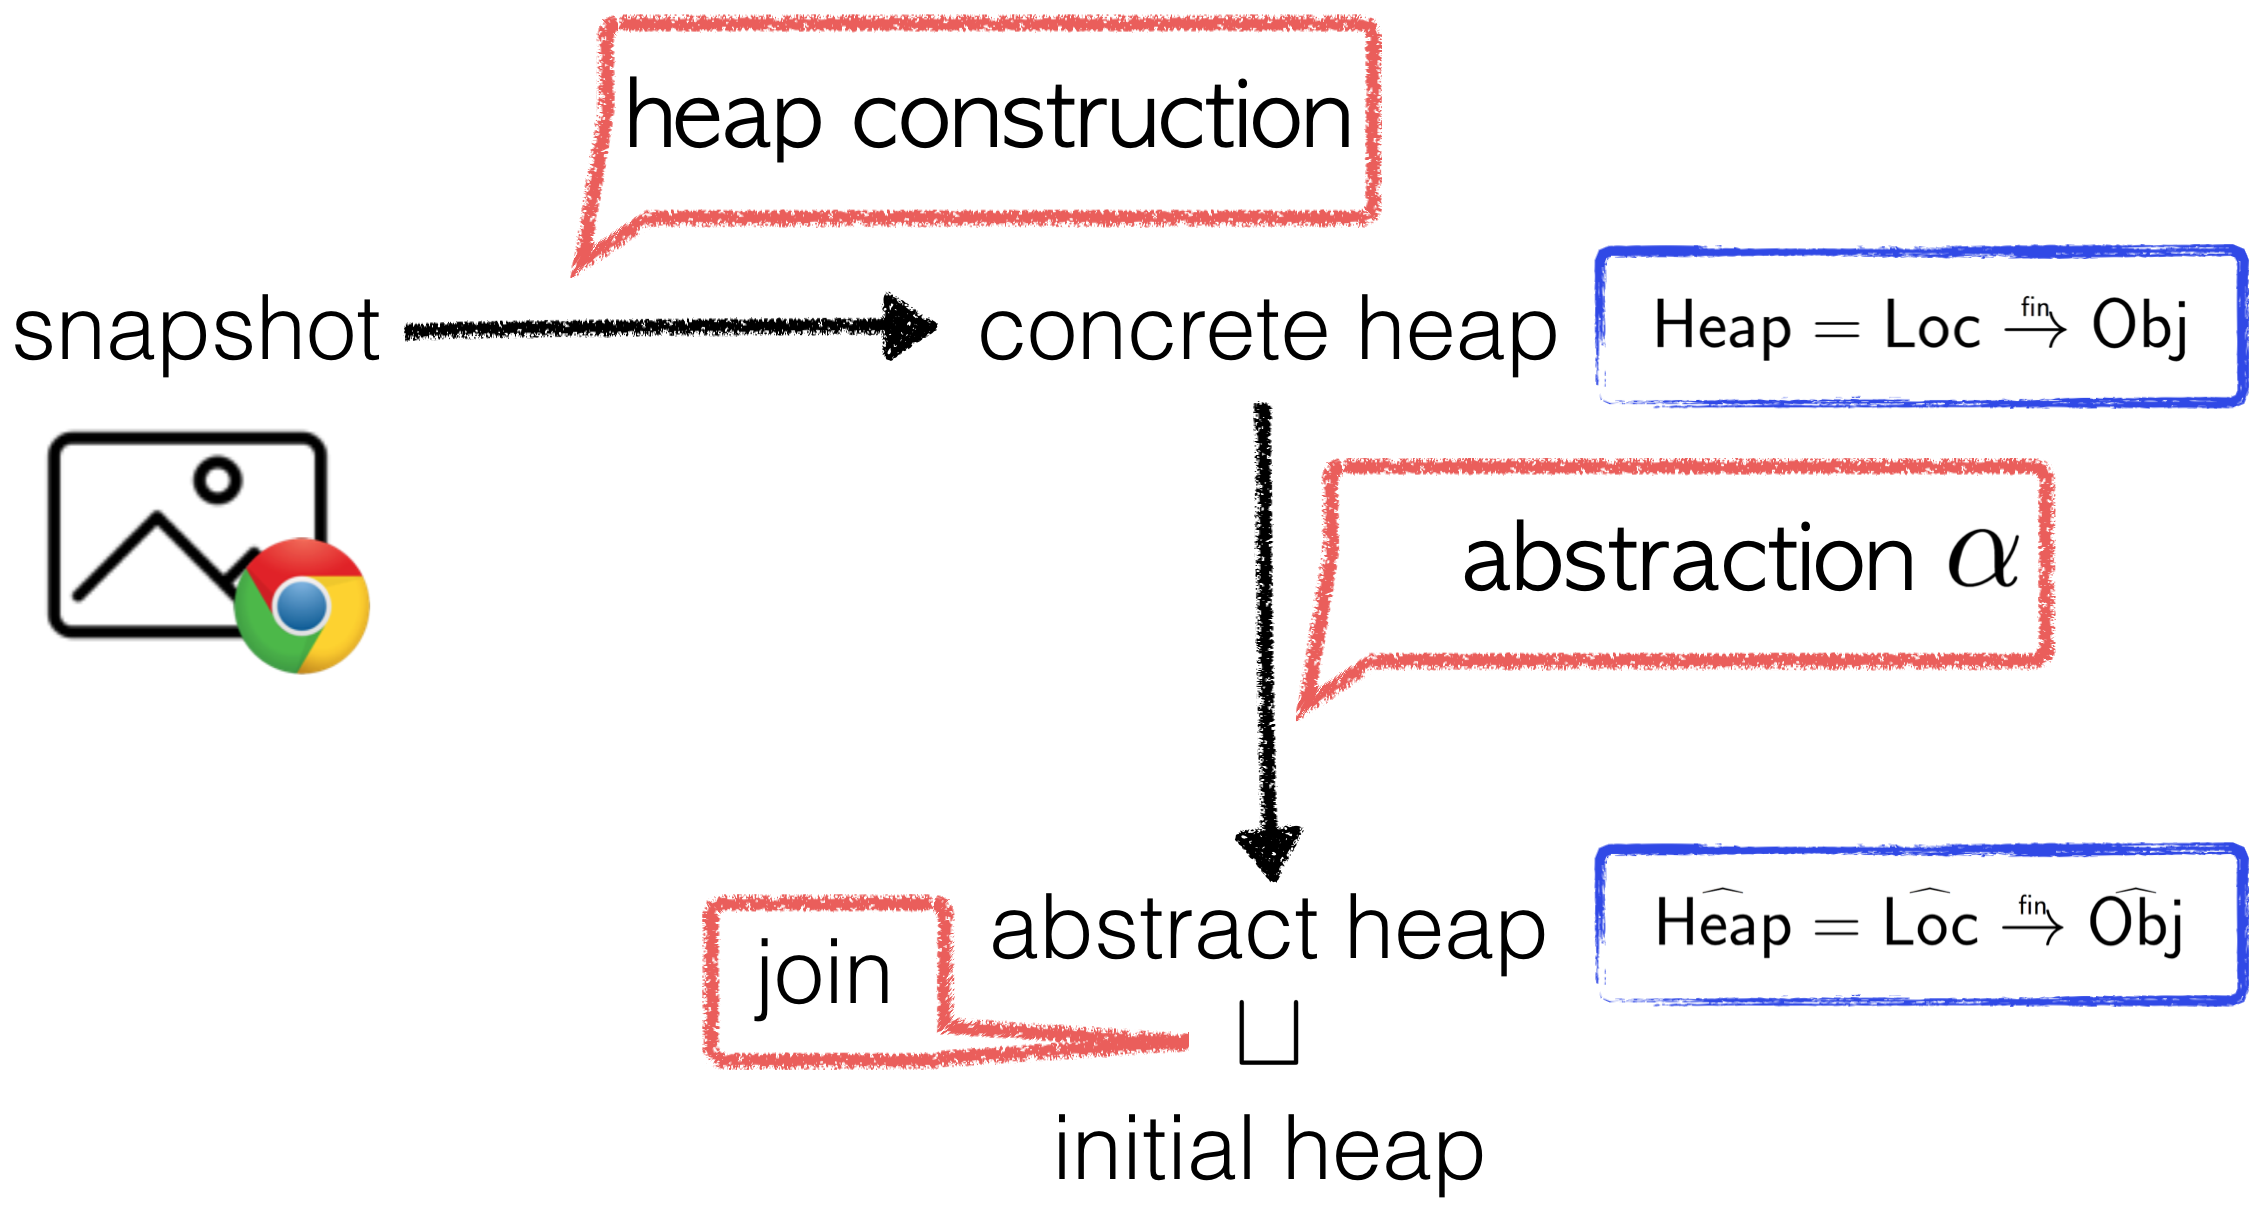
\includegraphics[width=\textwidth]{seip}
\end{minipage}
&
\begin{minipage}{.44\textwidth}
\small
\begin{verbatim}
sample snapshot
\end{verbatim}
\end{minipage}
\\\cline{2-2}
\end{tabular}
\vspace*{.5em}
\caption{\small Extension of \safe with dynamic heap information~\cite{safehybrid}}
\label{fig:seip}
\end{figure*}

Researchers may devise new analysis techniques or they may want to
reproduce analysis results reported in the literature.  In either way,
depending on which analysis technique is being implemented, one may
have to add a new phase or it may suffice to add one option to an
existing phase.  For example, when a researcher wanted to add
a simple symbolic executor to \oldsafe, the researcher had to modify
many functions in different files without much help from API functions.
In order to add a command, a phase, an option, a help message, and an
implementation of the new functionality, the researcher had to understand
many low-level details of \oldsafe.

Based on our own painful experiences, we revamped the structures of
the main \safe driver, commands, phases, options, and configurations,
and provide well-designed APIs for adding new commands, phases, and
options.  For example, when we extended \safe with a bug
detector~\cite{safewapp}, all we had to do was to make small
modifications in two files and to implement the bug detector.
Figure~\ref{fig:extensibility}(a) shows how we added a new command
\mtt{CmdBugDetect} and a new phase \mtt{BugDetect} in the main
driver file \mtt{Safe.scala}.  Figure~\ref{fig:extensibility}(b) presents
that we added the new command \mtt{CmdBugDetect} with a name
\mtt{bugDetect} and its phases \mtt{CmdAnalyze >> BugDetect},
which denotes that the new phase \mtt{BugDetect} is added to the end
of the phases of the command \mtt{CmdAnalyze}.  Then,
Figure~\ref{fig:extensibility}(c) shows the implementation of the
bug detector.  While the actual implementation is omitted at line 6,
simply providing its name, help message, configuration, and possible
options all in one single file is enough for \safe to plug the
information into appropriate places.  In this way, users do not
need to understand how \safe handles commands, phases, options, and
help messages, but they can simply specify what they are for the new
command.

Figure~\ref{fig:seip} illustrates another example that we extended \safe
with dynamic heap information as specified in the
literature~\cite{safehybrid}.  The technique is to capture the initial
concrete heap for each browser called \emph{snapshot}, to transform
it to its corresponding abstract heap, to merge the resulting
abstract heap with the default initial heap, and to use the merged heap
for the analysis.  Thus, the implementation of the technique consists
of two parts: a capturing app of concrete heaps, and code that
transforms a concrete heap to an abstract heap and merges it with another
abstract heap.  By using a browser-specific concrete heap
instead of a sound approximation that covers concrete heaps from
all the possible browsers, the technique reduces many false positives
from analysis results.  When applying the technique to \safe, we could
reuse the capturing app in tact, and we had to implement only 
\msf{heap construction} that parses a snapshot and constructs a concrete
heap in \safe, and we could reuse existing APIs for the remaining tasks.
As Figure~\ref{fig:seip} shows, for a given snapshot from the capturing
app, \msf{heap construction} constructs a concrete heap from the
snapshot.  Then, we can use the existing abstraction function for heaps
and the join operation on heaps in \safe.


\subsection{Debuggability}
While many programming language environments provide debugging
facilities, most static analysis frameworks do not provide such utilities
for analysis developers.  Because understanding and reasoning about
analysis status are extremely difficult, tracking the causes of analysis
imprecision is one of the active research topics.  However, existing
JavaScript analyzers are still in pre-mature stages.  \oldsafe provides
a console debugger, which allows users to investigte the analysis status
during analysis with stepwise exeuction of the underlying analyzer.
It indeed helps \oldsafe users debug the analyzer behaviors, but it lacks
documentation and it requires knowledge of the underlying analyzer.


To help \safe users to easily understand and reason about
analysis results, it now supports \htmldebug, which enables users
to investigate analysis status from browsers.  During analysis,
a user can write the current analysis status into an HTML file and
investigate it from a browser as illustrated in
Figure~\ref{fig:htmldebug}.  It shows the current CFG in the middle.
Nodes in black lines denote the blocks that are analyzed, those in
gray lines denote the blocks not yet being analyzed, and colored nodes
denote the blocks that are currently in the worklist of the analyzer.
One can toggle whether to show the nodes in the worklist by the menu
button on the top right.
When a user selects a block from the CFG, the list of the instructions in
the block and the state just before analyzing the block are displayed
on the left.


\safe has been tested using Test262, the official ECMAScript
conformance suite:
\begin{center}
\url{https://github.com/tc39/test262}
\end{center}
which helped us find and fix bugs in our modeling of builtin
functions specified in chapter 15 of the ECMAScript
specification~\cite{ECMA}.  Our regression test suite checks
whether the analysis results soundly approximate their corresponding
concrete values.  It also measures how many tests are being analyzed
precisely.  This test infrastructure with Test262 will aid \safe users
who build new analysis techniques to ``test'' the soundness and precision of their
new analysis implementation.


\begin{figure*}[t]
\centering
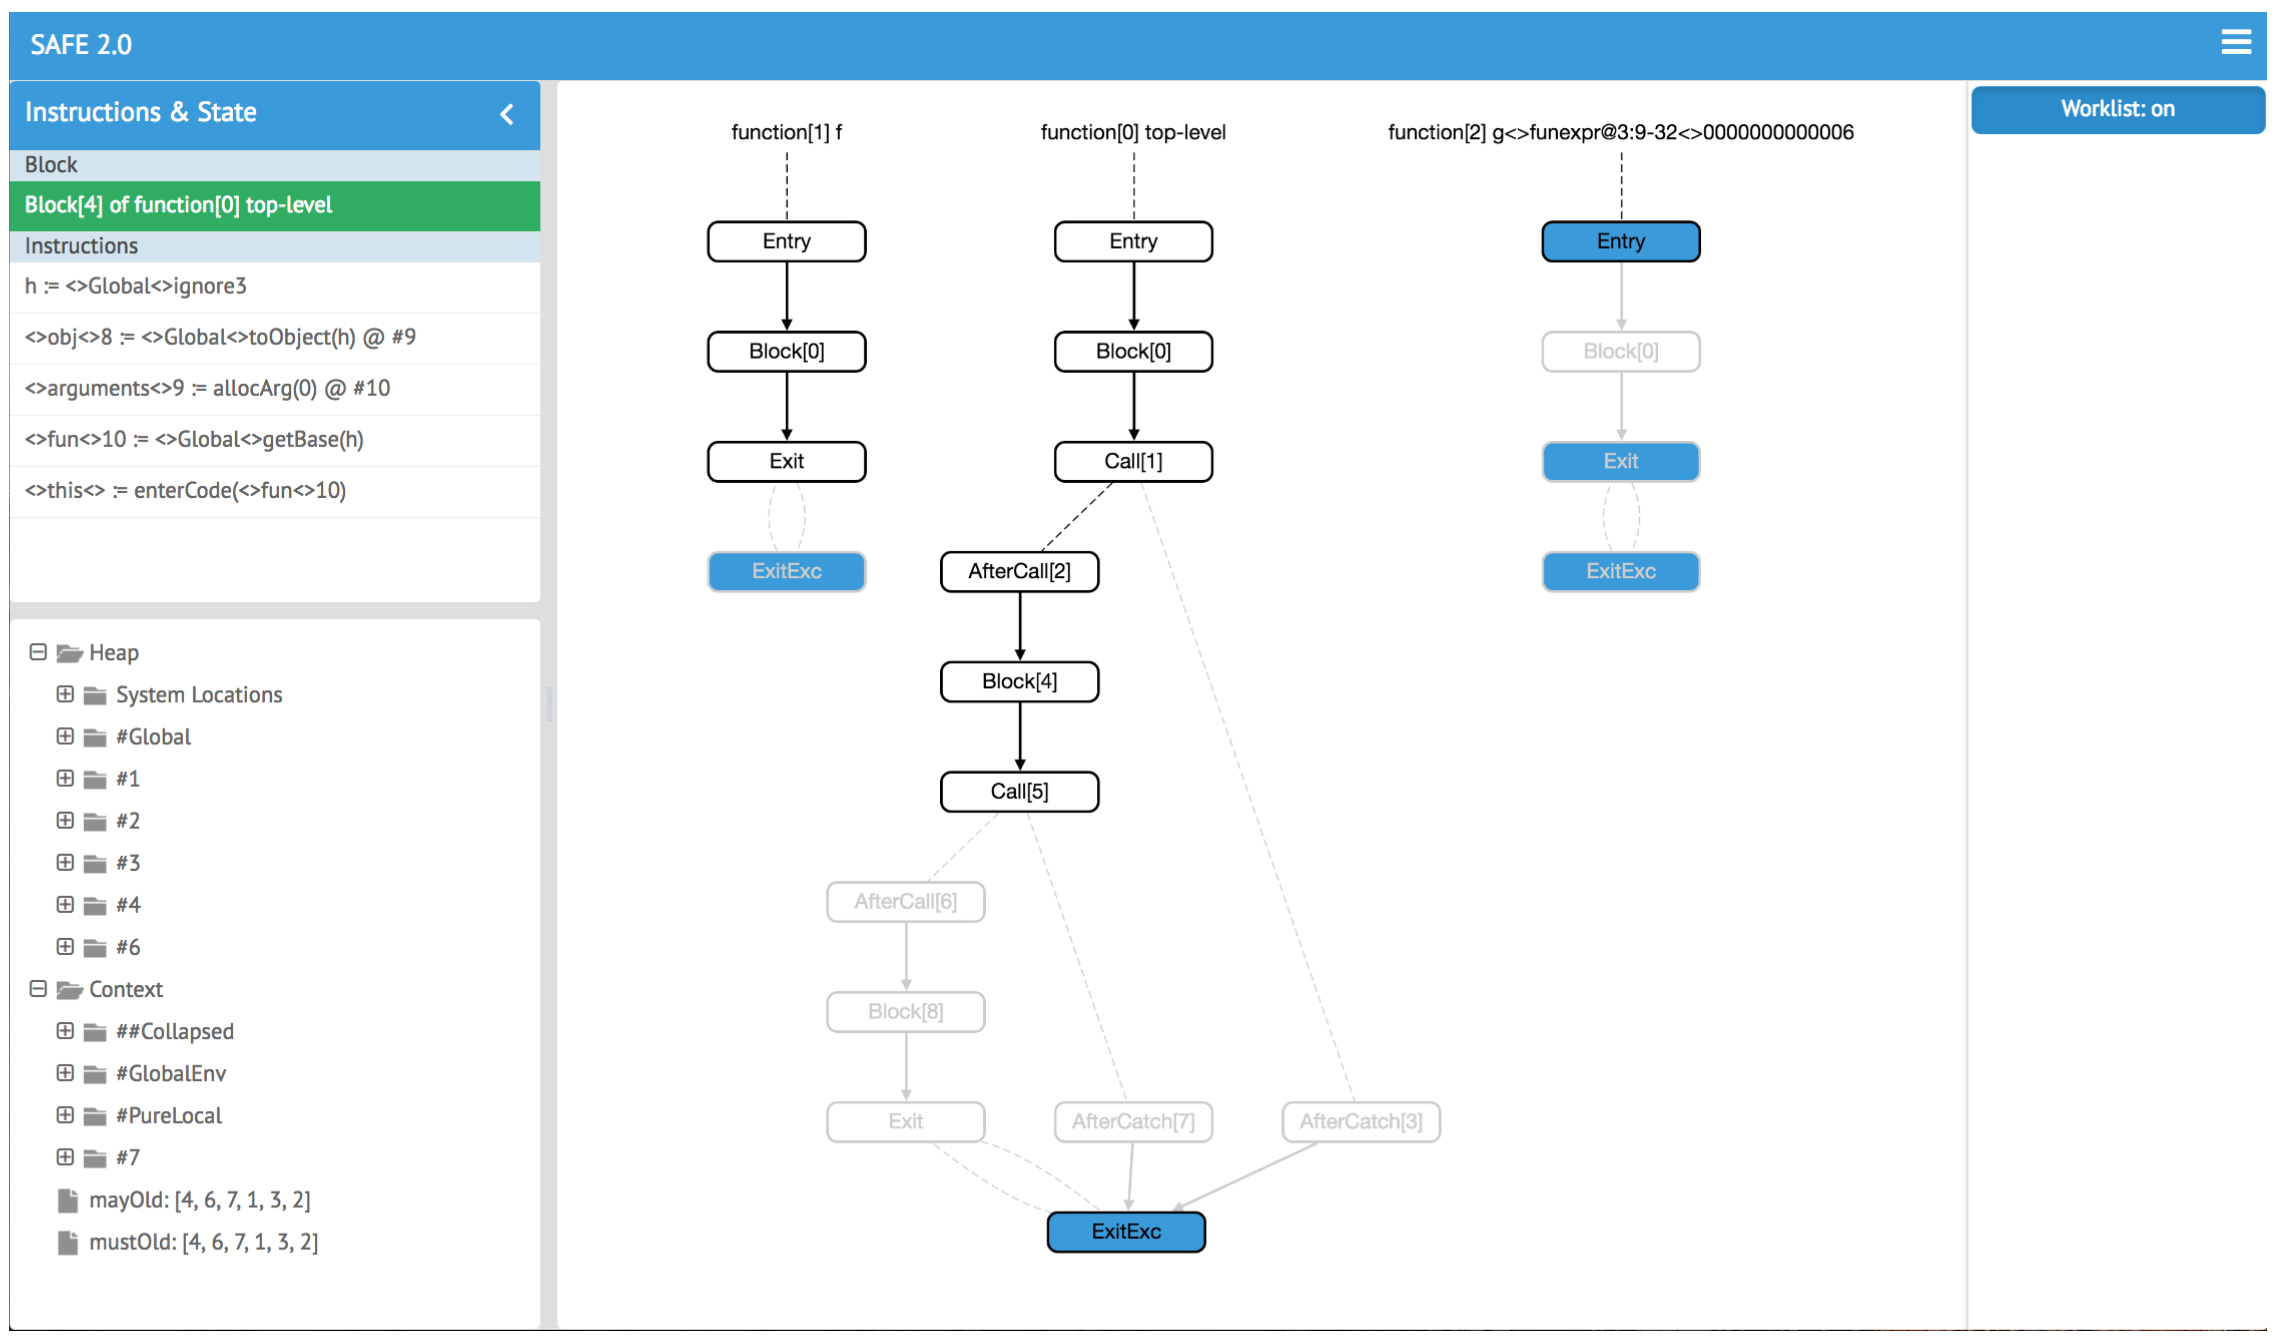
\includegraphics[width=.7\textwidth]{htmldebugger.png}
\caption{\htmldebug}\label{fig:htmldebug}
\end{figure*}

\section{Future Directions}
Since the release of \safe in early October 2016~\cite{saferelease},
we have been extending \safe with various features.
Among others, the following features will be supported in near future:
\begin{itemize}
\item Easier addition of sensitivities 
\item More support for abstract domain APIs
\item Improvements in \htmldebug

We are working on integration of the \safe analyzer and \htmldebug,
which would allow stepwise execution and more interactive debugging from browsers.
We plan to use a database for analysis results for scalability.
\end{itemize}
In addition, we plan to provide basic modeling supports for HTML/DOM
tree abstraction and the jQuery library, which has more than 90\% of
market share.  We believe \safe will let us explore more easily
the remaining challenges in analysis of JavaScript web applications
like event handling, modeling framework, and compositional analysis.


\section{Conclusion}
We present \safe, a tool that analyzes JavaScript web applications with
supports for analyzer users in mind.  On top of the well-tested core
features of \safe based on the prior experiences from building \oldsafe,
it also provides mechanisms for analysis developers to experiment with
their novel ideas without too much implementation burden.
It allows users to specify target phases and options in a declarative
manner, which can configure even abstract domains and analysis
sensitivities.  Analyzer developers can add new analysis techniques
into \safe without too much understanding of the implementation details
of \safe via its extensible APIs.  Finally, \safe provides a debugging
support for analysis developers with visualization and interactive
investigation of the analysis status.  The tool was motivated by the pain
the authors themselves experienced with \oldsafe, which was greatly
relieved by the \htmldebug.  Also, analysis developers can test their
new analysis techniques with extensive Test262, the official ECMAScript
conformance suite.

\bibliographystyle{abbrv}
\bibliography{ref}
\end{document}
